% xelatex

\documentclass[a4paper,10pt]{article}

\usepackage{marvosym}
\usepackage{fontspec} 					%for loading fonts
\usepackage{xunicode,xltxtra,url,parskip} 		%other packages for formatting
\RequirePackage{color,graphicx}
\usepackage[usenames,dvipsnames]{xcolor}
\usepackage{fullpage}                                   % alternative to layaureo
%\usepackage[big]{layaureo} 				%better formatting of the A4 page
%\usepackage{fullpage}					%standard margines
%\usepackage{supertabular} 				%for Grades
\usepackage{titlesec}					%custom \section
\usepackage[none]{hyphenat}				%disable any hyphenation
\usepackage{graphicx}					%photo import
\usepackage{wrapfig}					%image/text wrapping
\usepackage{hyperref}					%setup hyperref package, and colours for links
\usepackage{setspace}					%setup line spacing
\usepackage{array}					%table lines
\usepackage{ulem}					%underlining: for big correct underline distance

\setlength{\parskip}{\baselineskip}

%\definecolor{linkcolor}{rgb}{0,0.2,0.6}
%\definecolor{linkcolor}{rgb}{.1,.4,.9}
%\definecolor{linkcolor}{rgb}{.1,.3,.7}
\definecolor{linkcolor}{RGB}{10, 40, 155}
\definecolor{mygray}{gray}{0.25}
\definecolor{linegray}{gray}{0.6}

\def\name{Petar I. Ivanov}
\def\myline{\color{linegray}\vline}
\def\interestsSpace{\\[1.3mm]}				%wider line spacing

\newcommand{\minorcolor}[1]{\textcolor{mygray}{#1}}
\newcommand{\wide}{\addfontfeature{LetterSpace=3.0}}	%wide letter spacing

\hypersetup{
  colorlinks = true,
%  urlcolor = black,
  urlcolor = linkcolor,
  pdfauthor = {\name},
  pdfkeywords = {Computer Science},
  pdftitle = {\name: Curriculum Vitae},
  pdfsubject = {Curriculum Vitae},
  pdfpagemode = UseNone
}

%FONTS
\defaultfontfeatures{Mapping=tex-text}
\setmainfont[SmallCapsFont = Fontin SmallCaps]{Fontin}

%CV Sections
\titleformat{\section}{\Large\scshape\raggedright}{}{0em}{}[\color{linegray}\titlerule]	% section style
\titlespacing{\section}{0pt}{10pt}{0pt}

% MARGINES
\addtolength{\oddsidemargin}{-3mm}
\addtolength{\evensidemargin}{-3mm}
\addtolength{\textwidth}{8mm}

\addtolength{\topmargin}{5mm}
\addtolength{\textheight}{25mm}

\linespread{1.15}				%line spacing

%--------------------BEGIN DOCUMENT----------------------
\begin{document}
\pagestyle{empty}				% non-numbered pages
\font\fb=''[cmr10]''				%for use with \LaTeX command

% *** Photo ***
\begin{wrapfigure}{r}{3.5cm}
	\setlength\fboxsep{0pt}
	\setlength\fboxrule{0.1pt}
	\vspace{-20pt}\fbox{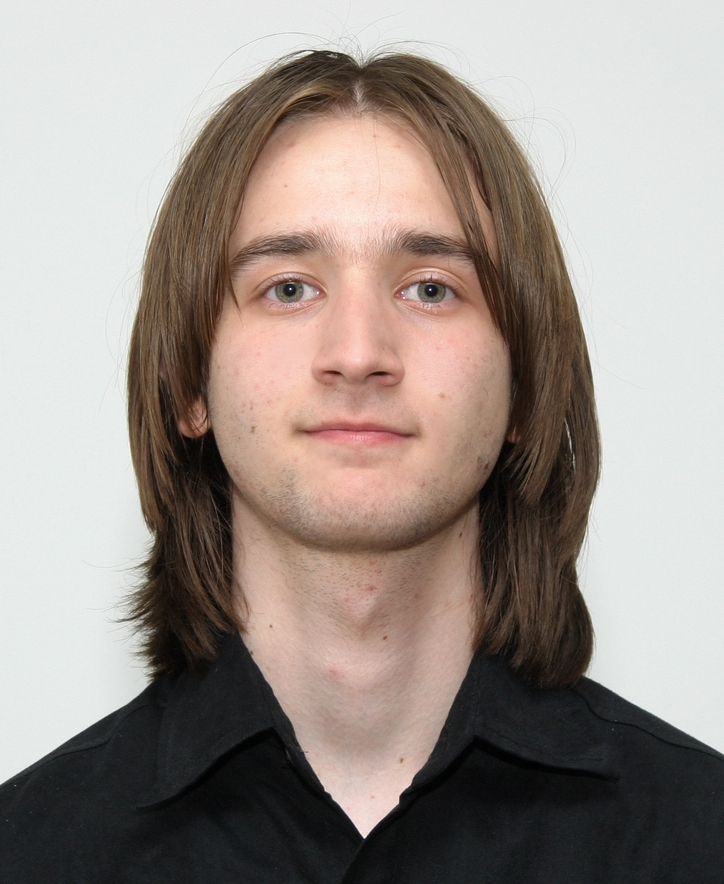
\includegraphics[width=33mm]{PetarIvanov.jpg}}
\end{wrapfigure}

% *** Profile ***
\par{\raggedright\Huge\textbf{\vspace{-3mm}\hspace{0mm}\name}}\\		% big name on the top
\vspace{-5mm}{\color{linegray}\rule{10.5cm}{0.1mm}}\\

\hspace{4mm}\begin{tabular}{rl}
	\minorcolor{Born:} & \textsc{29 May 1989} in Shumen, Bulgaria\\
	\minorcolor{Address:} & \textsc{1} Leninskie gory, B-737, Moscow \textsc{119192}, Russia\\
	\minorcolor{Phone:} & \textsc{+7 (963) 929-10-52}\\
	\minorcolor{E-mail:} & \href{mailto:peter.ivanov89@gmail.com}{peter.ivanov89@gmail.com}\\
\end{tabular}
\bigskip

%Section: *** Education ***
\section{Education}
\hspace{0mm}\begin{tabular}{r!{\myline}p{14cm}}
	\textsc{2011 -- 2013}     &  Student {\small\textit{(1\textsuperscript{st} year out of 2)}} in \textsc{Bioinformatics}\\
	\small\textit{(current)}  &  \textbf{Yandex's School of Data Mining}, Russia\\
	
        \multicolumn{2}{c}{}\\
        \textsc{2009 -- 2014}     &  Specialist degree {\small\textit{(4\textsuperscript{th} year out of 5)}} in \textsc{Applied Mathematics and Informatics}\\
        \small\textit{(current)}  &  Major in Stereo vision \& Robotics, \textsc{Graphics \& Media laboratory}\\
                                  &  \textit{Faculty of Computational Mathematics and Cybernetics}\\
                                  &  \textbf{Moscow State University}, Russia\\
                                  %&  \textsc{Gpa}: 4.00/5 \\ 
                                  %{\small\textit{exp.}}

	\multicolumn{2}{c}{}\\
	\textsc{2008 -- 2009}     &  Bachelor degree {\small\textit{(1\textsuperscript{st} year)}} in \textsc{Computer science}\\
                                  &  \textit{Faculty of Mathematics and Informatics}\\
                                  &  \textbf{Sofia University}, Bulgaria\\
                                  %&  \textsc{Gpa}: 5.57/6 \\
	
	\multicolumn{2}{c}{}\\
	\textsc{2000 -- 2008}     &  Mathematics and Physics class\\
                                  &  \textit{Graduated with honors}\\ %\textsc{Golden prize for High Achievements}\\
                                  &  \textbf{High school of Natural Sciences and Mathematics}, Shumen, Bulgaria\\
                                  %&  \textsc{Gpa}: 5.92/6 \\
\end{tabular}
\par\smallskip

\hspace{7mm}{\textit{\minorcolor{\underline{Additional:}}}

\hspace{0mm}\begin{tabular}{r!{\myline}p{14cm}}
	\textsc{Jan 2011}       &  \textsc{Vision and Machine-learning Research School}, ENS Lyon, France\\
	\textsc{Jul 2008}       &  \textsc{Russian Summer Informatics Camp}, Sudislavl, Kostroma region, Russia\\
	\textsc{Aug 2007}       &  \textsc{Physics Camp}, Panitsite region, Bulgaria\\ % without TEO !!!
	\textsc{2004 -- 2007}   &  \textsc{Summer Research Informatics Camp}, Varna, Bulgaria\\
	\textsc{2001 -- 2008}   &  \textsc{Mathematics and Informatics Private School ``A\&B''}, Shumen, Bulgaria\\
\end{tabular}

\hspace{7mm}\textit{\minorcolor{\underline{Complementary courses passed:}}}

\hspace{1.5mm}\begin{tabular}{r!{\myline}p{5cm}r!{\myline}p{6cm}}
  	 \minorcolor{Moscow}  &  \textsc{Image Processing}      &          \minorcolor{Sofia} & \textsc{Computational Geometry}\\
 	  \minorcolor{State}  &  \textsc{Video Processing}      &     \minorcolor{University} & \textsc{Computational Linguistics}\\
     \minorcolor{University}  &  \textsc{Computer Vision}\\
	                      &  \textsc{Combinatorial Optimization}\\
	                      &  \textsc{Bioinformatics Tools}\\
\end{tabular}

\newpage
%Section: *** Awards ***
\section{Awards}
\par{\vspace{-9mm}\hspace{7cm}{\minorcolor{\textit{the competitions are National Bulgarian if nothing else stated}}}}\\

\vspace{-3mm}\hspace{3.5mm}\begin{tabular}{r!{\myline}p{14cm}}
	I\textsuperscript{st} place    &  \textsc{``Minko Balkanski''} \textsc{Competition in Informatics} \textsc{'08}\\
	XI\textsuperscript{th} place   &  \textsc{TopCoder High School Finals}, West Lafayette, USA \textsc{'08}\\
	I\textsuperscript{st} place    &  \textsc{Autumn Tournament in Informatics} \textsc{'07}\\
	I\textsuperscript{st} place    &  Student Competition for the \textsc{Dean's cup of Sofia University} \textsc{'07}\\
	II\textsuperscript{nd} place   &  \textsc{International Young Physicists Tournament} {\small\textit{(regional, in team)}} \textsc{'06}\\
	I\textsuperscript{st} place    &  \textsc{``Rumen Grozdanov''} \textsc{Informatics and Mathematics Tournament} \textsc{'06}\\
	I\textsuperscript{st} place    &  \textsc{Winter Tournament in Informatics} \textsc{'06}\\
\end{tabular}
\medskip

\hspace{3mm}\begin{tabular}{@{•\enskip}p{14.5cm}}
%\setlength{\parindent}{1cm}
	Awarded as a \textsc{National Laureate in Informatics}, Bulgaria, \textsc{'08}\\
	Classed for the \underline{final rounds} of the \textsc{Bulgarian Olympiad in Informatics}, from \textsc{'05} to \textsc{'08} \small\textit{(incl.)}\\
	Participant in the \textsc{TopCoder High School Finals}, West Lafayette, USA \textsc{'07} and \textsc{'08}\\
	Classed for the \underline{final rounds} of \textsc{``Musala Soft and PC Magazine''} competition in \textsc{'07} and \textsc{'08}\\
%	Participated in the tournament \textsc{Australian Mathematics Trust} from \textsc{2005} to \textsc{2007}\\
\end{tabular}

%\medskip
%\hspace{3mm}\begin{tabular}{@{--- }p{14.5cm}}
%	Scholarship for \textit{science achievements} of \textsc{American Foundation for Bulgaria} in \textsc{'07} and \textsc{'08}\\
%	Scholarship for \textit{excellent grades} in \textsc{'06}, \textsc{'07} and \textsc{'08}\\
%\end{tabular}

%Section: *** Work Experience ***
\section{Work Experience}
\hspace{0mm}\begin{tabular}{r!{\myline}p{14cm}}
        %\multicolumn{2}{c}{}\\
	\textsc{Sep 2012 --}      &  \textit{Mathematics consultant and programmer of cellular models}\\
        \small\textit{(current)}  &  supervised by prof. Konstantin Severinov, Molecular Genetics of Microorganisms Lab\\
                                  &  \textbf{Institute of Gene biology, Russian Academy of Sciences} (\href{http://www.genebiology.ru/}{genebiology.ru})\\
	
        \multicolumn{2}{c}{}\\
	\textsc{Jul 2012 --}      &  \textit{Researcher into verification of probabilistic biological models}\\
        \textsc{Aug 2012} &  supervised by prof. Martin Vechev, \textbf{Software Reliability Lab}\\
                                  &  \textbf{ETH Zurich} (\href{http://www.srl.inf.ethz.ch/}{srl.inf.ethz.ch}), Switzerland\\
	
        \multicolumn{2}{c}{}\\
	\textsc{Jul 2011 --}      &  \textit{Open source developer of local topological operators on tetrahedral meshes}\\
	\textsc{Aug 2011}         &  \textbf{Computational Geometry Algorithms Library (CGAL)} (\href{http://www.cgal.org/}{cgal.org})\\
                                  &  \textbf{Google Summer of Code} (\href{http://code.google.com/soc/}{code.google.com/soc})\\
	
        \multicolumn{2}{c}{}\\
	\textsc{Aug 2010}         &  \textit{Lecturer}\\
	                          &  \textbf{Russian Summer Informatics Camp} (\href{http://lksh.ru/}{lksh.ru}), Saratov, Russia\vspace{-5mm}\\
	
	\multicolumn{2}{c}{}\\
	\textsc{Mar 2008 --}      &  \textit{Assistant in \textsc{``Design and Analysis of Algorithms''} course}\\
	\textsc{June 2009}        &  \textbf{Faculty of mathematics and informatics, Sofia University}, Bulgaria\\

	\multicolumn{2}{c}{}\\
	\textsc{Sept 2008 --}     &  \textit{Jury, organizer, tester and \textit{author} of the problems in}\\
	\textsc{June 2009}        &  \textsc{on-line programming tournament} (\href{http://konkurs.musala.com/}{konkurs.musala.com})\\
	                          &  \textbf{Musala Soft}, Sofia, Bulgaria\\

	\multicolumn{2}{c}{}\\
	\textsc{Sept 2008 --}     &  \textit{Author of problems in all} \textsc{Bulgarian Tournaments in Informatics}\\
	\textsc{June 2009}        &  \textit{Lecturer in the} \textsc{National Informatics Camps}\\
                                  &  \textbf{National Committee in Informatics}, \textbf{Bulgarian Ministry of Education}\\

	\multicolumn{2}{c}{}\\
	\textsc{July 2007 --}     &  \textit{Developer of a bin-packing genetic algorithm for glass cutting optimization}\\
	\textsc{Sept 2007}        &  \textbf{Telepol Net} (\href{http://telepol.com/}{telepol.com}), Shumen, Bulgaria\\
	
\end{tabular}

\newpage
%Section: *** Languages ***
\section{Spoken languages}
\hspace{1mm}\begin{tabular}{rp{14cm}}
	\textsc{English:}     &  Upper-Intermediate {\small\textit{(certified)}}\\
	\textsc{Russian:}     &  Fluent {\small\textit{(certified)}}\\
	\textsc{Bulgarian:}   &  Native\\
\end{tabular}

%Section: *** Computer Skills ***
\section{Information technologies}
\hspace{2.5mm}\begin{tabular}{rp{14cm}}
        Languages:      &  \textbf{C\,/\,C++ (STL)}, \textsc{Python (NumPy, SciPy),\,\,Matlab,\,\,Java,\,\,Pascal,\,\,Assembler,\,\,HTML,\,\,PHP,\,\,{\fb \LaTeX}}\\
        Technologies:   &  \textsc{Unix, Vim}\\
\end{tabular}

%Section: *** Interests and Activities ***
\section{Activities}
\hspace{2mm}\begin{tabular}{@{•\enskip}p{14.5cm}}
%	\setlength{\parindent}{1cm}
%	Scientifically interested in \textsc{Computer Vision, Computational Geometry, Bioinformatics, Machine Learning, Genetic Algorithms}\interestsSpace	
        Scientifically interested in:\newline
	\begin{tabular}{@{--- \enskip}p{14.5cm}}
		Bioinformatics\\
		Computer Vision\\
		Computational Geometry\\
		Genetic Algorithms\\
		Machine Learning\\
	\end{tabular}\interestsSpace
	Solving algorithmical problems (\href{http://www.topcoder.com/tc?module=MemberProfile&cr=10205233}{\textsc{TopCoder}}, \href{http://acm.timus.ru/author.aspx?id=30642}{\textsc{Timus}}, \href{http://rosalind.info/users/cheater_no1/}{\textsc{Rosalind}})\interestsSpace
        Going more open sourced (\href{https://github.com/petar-ivanov/}{\textsc{code}}, \href{https://opensnp.org/users/637}{\textsc{23andme genotype}})\interestsSpace
        Founder of the \href{http://students-abroad.info/}{\textsc{Students-abroad project}} for describing some foreign educational systems by Bulgarians studying abroad including my own \href{http://pesho.info/category/msu}{\textsc{blog}} about Moscow State University\interestsSpace
%In process of internationalizing the \textsc{Bulgarian Summer Research Informatics Camp}: organizing the participation of Russian students in \textsc{2011}\interestsSpace
	%Universally interested in {\wide Evolution and Linguistics}\interestsSpace
        Practicing {\wide hiking, orienteering, long-distance running}
        (\href{http://probeg.org/card.php?id=273}{Dec 2011, Zelenograd, Russia} -- 42.195km~in~3:43h; \href{http://www.vitosha100km.bg/2011/}{Jul 2012, Vitosha mountain, Bulgaria} -- 100km~in~13:19h)\interestsSpace
\end{tabular}

%\vspace{0mm}
%Section: *** References ***
%\section{References}
%\vspace{-6mm}\hspace{11cm}{\minorcolor{\textit{university teachers of mine}}}\\

%\vspace{-3mm}\hspace{-1mm}\begin{tabular}{llp{4.5cm}}
%	{\textbf {Prof. {\large Krassimir Manev}, PhD}} & {\textbf {PhD {\large Dmitriy Vatolin}}} & {\textbf{PhD {\large Anton Konushin}}}\\
%	\textsc{Discrete Mathematics}& \textsc{Video processing and {\addfontfeature{LetterSpace=-14.0}Compression}} & \textsc{Computer Vision}\\
%	\vspace{2mm}
%	\textit{International Committee of IOI} & \textit{Head of MSU Video group} & \textit{Head of MSU Vision group}\\
%	\textbf{Sof{}ia University} & \textbf{Moscow State University} & \textbf{Moscow State University}\\
%	\href{mailto:manev@fmi.uni-sofia.bg}{manev@fmi.uni-sofia.bg} & \href{mailto:dmitriy@graphics.cs.msu.ru}{dmitriy@graphics.cs.msu.ru} & \href{mailto:ktosh@graphics.cs.msu.ru}{ktosh@graphics.cs.msu.ru}\\
%	\textsc{+359 (887) 25-32-11} & \textsc{+7 (903) 762-82-87} & \textsc{+7 (916) 620-31-85}\\
%\end{tabular}

%\smallskip
%\quad \minorcolor{\textit{* \small the references are university teachers of mine}}

%	• & Iskren Chernev -- \textbf{Sofia University} -- \href{mailto:iskren.chernev@gmail.com}{iskren.chernev@gmail.com} -- the person who informally best knows my ambitions -- Googler '09\\
%	• & Alexander Dainiak -- \textbf{Moscow State University} -- \href{mailto:dainiak@gmail.com}{dainiak@gmail.com} -- Discrete Mathematics researcher\\

\end{document}
